\documentclass[11pt,a4paper]{jsarticle}
\usepackage{amsmath,amssymb}
\usepackage{amsthm}
\usepackage{ascmac}
\usepackage{bm}
\usepackage[dvipdfmx]{graphicx}	% required for `\includegraphics' (yatex added)
\usepackage{setspace}           % required for `\doublespace'
\usepackage{tikz}
\usepackage{tikz-cd}
\usetikzlibrary{angles, positioning, shapes, arrows.meta, decorations.pathmorphing}
%\usetikzlibrary{intersections, calc, arrows, positioning, arrows.meta}
\usepackage{tcolorbox}  % 定理環境の装飾
\tcbuselibrary{skins, breakable, theorems}
\usepackage{xcolor}
\usepackage{natbib}
\usepackage{pxrubrica}
\usepackage[margin=30truemm, left=40truemm, right=40truemm]{geometry}
\usepackage{thmbox}     % required for theorem environment with side bar
%
\setlength{\parskip}{3mm} %段落間にスペースを入れる


% \pagestyle{myheadings}
% \markright{\footnotesize \sf 2022秋期「哲学者のための数学」授業資料(大塚淳) \ \ 配布禁止}


\theoremstyle{definition}
\newtheorem[S]{exercise}{練習問題}[section]
\newtheorem[S]{example}{事例}[section]
\newtheorem[S]{fact}{事実}[section]
\newtheorem[S]{attn}{注意}[section]
\newtheorem[S]{develop}{発展}[section]
\renewcommand{\theattn}{}

\newtcbtheorem[auto counter, number within=section]{rei}{事例}{
    breakable,
    coltitle=black,
    fonttitle=\bfseries,
    enhanced, colback=white, frame hidden, borderline west = {0.5pt}{5pt}{black},
%    number freestyle={\noexpand\thesection.\noexpand\arabic{\tcbcounter}}
}{rei}

\newtcbtheorem[auto counter, number within=section]{prop}{命題}{
    breakable,
    coltitle=black,
    fonttitle=\bfseries,
    enhanced, colback=white, frame hidden, borderline west = {0.5pt}{5pt}{black},
%    number freestyle={\noexpand\thesection.\noexpand\arabic{\tcbcounter}}
}{prop}

\newtcbtheorem[number within=section]{renshu}{練習問題}{
    breakable,
    coltitle=black,
    fonttitle=\bfseries,
    enhanced, colback=white, frame hidden, borderline west = {0.5pt}{5pt}{black}
}{renshu}


\newtcbtheorem[number within=section]{hatten}{発展}{
    breakable,
    coltitle=black,
    fonttitle=\bfseries,
    enhanced, colback=white, frame hidden, borderline west = {0.5pt}{5pt}{black}
}{renshu}


\newtcbtheorem[number within=section]{dfn}{定義}{
    fonttitle=\bfseries,
    enhanced, colback=white
}{dfn}


% Bold face capital letters:
\newcommand{\bfzero}{\boldsymbol{0}}
\newcommand{\bfone}{\boldsymbol{1}}
\newcommand{\bfA}{\boldsymbol{A}}
\newcommand{\bfB}{\boldsymbol{B}}
\newcommand{\bfC}{\boldsymbol{C}}
\newcommand{\bfD}{\boldsymbol{D}}
\newcommand{\bfE}{\boldsymbol{E}}
\newcommand{\bfF}{\boldsymbol{F}}
\newcommand{\bfG}{\boldsymbol{G}}
\newcommand{\bfH}{\boldsymbol{H}}
\newcommand{\bfI}{\boldsymbol{I}}
\newcommand{\bfJ}{\boldsymbol{J}}
\newcommand{\bfK}{\boldsymbol{K}}
\newcommand{\bfL}{\boldsymbol{L}}
\newcommand{\bfM}{\boldsymbol{M}}
\newcommand{\bfN}{\boldsymbol{N}}
\newcommand{\bfO}{\boldsymbol{O}}
\newcommand{\bfP}{\boldsymbol{P}}
\newcommand{\bfQ}{\boldsymbol{Q}}
\newcommand{\bfR}{\boldsymbol{R}}
\newcommand{\bfS}{\boldsymbol{S}}
\newcommand{\bfT}{\boldsymbol{T}}
\newcommand{\bfU}{\boldsymbol{U}}
\newcommand{\bfV}{\boldsymbol{V}}
\newcommand{\bfW}{\boldsymbol{W}}
\newcommand{\bfX}{\boldsymbol{X}}
\newcommand{\bfY}{\boldsymbol{Y}}
\newcommand{\bfZ}{\boldsymbol{Z}}

\newcommand{\bfa}{\boldsymbol{a}}
\newcommand{\bfb}{\boldsymbol{b}}
\newcommand{\bfc}{\boldsymbol{c}}
\newcommand{\bfd}{\boldsymbol{d}}
\newcommand{\bfe}{\boldsymbol{e}}
\newcommand{\bff}{\boldsymbol{f}}
\newcommand{\bfk}{\boldsymbol{k}}
\newcommand{\bfm}{\boldsymbol{m}}
\newcommand{\bfn}{\boldsymbol{n}}
\newcommand{\bfo}{\boldsymbol{o}}
\newcommand{\bfp}{\boldsymbol{p}}
\newcommand{\bfq}{\boldsymbol{q}}
\newcommand{\bfr}{\boldsymbol{r}}
\newcommand{\bfs}{\boldsymbol{s}}
\newcommand{\bft}{\boldsymbol{t}}
\newcommand{\bfu}{\boldsymbol{u}}
\newcommand{\bfv}{\boldsymbol{v}}
\newcommand{\bfw}{\boldsymbol{w}}
\newcommand{\bfx}{\boldsymbol{x}}
\newcommand{\bfy}{\boldsymbol{y}}
\newcommand{\bfz}{\boldsymbol{z}}



% BB (???) capital letters:
\newcommand{\bbA}{\mathbb{A}}
\newcommand{\bbB}{\mathbb{B}}
\newcommand{\bbC}{\mathbb{C}}
\newcommand{\bbD}{\mathbb{D}}
\newcommand{\bbE}{\mathbb{E}}
\newcommand{\bbF}{\mathbb{F}}
\newcommand{\bbG}{\mathbb{G}}
\newcommand{\bbI}{\mathbb{I}}
\newcommand{\bbN}{\mathbb{N}}
\newcommand{\bbP}{\mathbb{P}}
\newcommand{\bbQ}{\mathbb{Q}}
\newcommand{\bbR}{\mathbb{R}}
\newcommand{\bbU}{\mathbb{U}}
\newcommand{\bbV}{\mathbb{V}}
\newcommand{\bbX}{\mathbb{X}}
\newcommand{\bbY}{\mathbb{Y}}
\newcommand{\bbZ}{\mathbb{Z}}
\newcommand{\bbone}{{\ifmmode\mathrm{1\!l}\else\mbox{\(\mathrm{1\!l}\)}\fi}}


% Caligraphic math capital letters:
\newcommand{\mcalA}{\mathcal{A}}
\newcommand{\mcalB}{\mathcal{B}}
\newcommand{\mcalC}{\mathcal{C}}
\newcommand{\mcalD}{\mathcal{D}}
\newcommand{\mcalE}{\mathcal{E}}
\newcommand{\mcalF}{\mathcal{F}}
\newcommand{\mcalG}{\mathcal{G}}
\newcommand{\mcalH}{\mathcal{H}}
\newcommand{\mcalI}{\mathcal{I}}
\newcommand{\mcalJ}{\mathcal{J}}
\newcommand{\mcalK}{\mathcal{K}}
\newcommand{\mcalL}{\mathcal{L}}
\newcommand{\mcalM}{\mathcal{M}}
\newcommand{\mcalN}{\mathcal{N}}
\newcommand{\mcalO}{\mathcal{O}}
\newcommand{\mcalP}{\mathcal{P}}
\newcommand{\mcalQ}{\mathcal{Q}}
\newcommand{\mcalS}{\mathcal{S}}
\newcommand{\mcalT}{\mathcal{T}}
\newcommand{\mcalU}{\mathcal{U}}
\newcommand{\mcalV}{\mathcal{V}}
\newcommand{\mcalX}{\mathcal{X}}
\newcommand{\mcalY}{\mathcal{Y}}
\newcommand{\mcalZ}{\mathcal{Z}}

% Graph nodes notations:
\newcommand{\PA}{\mathit{PA}}
\newcommand{\bfPA}{\mathbf{PA}}
\newcommand{\CH}{\mathit{CH}}
\newcommand{\bfCH}{\mathbf{CH}}
\newcommand{\DS}{\mathit{DS}}
\newcommand{\bfDS}{\mathbf{DS}}
\newcommand{\ND}{\mathit{ND}}
\newcommand{\bfND}{\mathbf{ND}}
\newcommand{\AN}{\mathit{an}}
\newcommand{\bfAN}{\mathbf{an}}
\newcommand{\pa}{\mathit{pa}}
\newcommand{\bfpa}{\mathbf{pa}}
\newcommand{\ch}{\mathit{ch}}
\newcommand{\bfch}{\mathbf{ch}}
\newcommand{\ds}{\mathit{ds}}
\newcommand{\bfds}{\mathbf{ds}}
\newcommand{\nd}{\mathit{nd}}
\newcommand{\bfnd}{\mathbf{nd}}
\newcommand{\an}{\mathit{an}}
\newcommand{\bfan}{\mathbf{an}}



\DeclareMathOperator*{\argmax}{arg\,max}
\DeclareMathOperator*{\argmin}{arg\,min}
\DeclareMathOperator*{\argsup}{arg\,sup}
\DeclareMathOperator*{\arginf}{arg\,inf}
\DeclareMathOperator{\erfc}{erfc}
\DeclareMathOperator{\diag}{diag}
\DeclareMathOperator{\cum}{cum}
\DeclareMathOperator{\sgn}{sgn}
\DeclareMathOperator{\tr}{tr}
\DeclareMathOperator{\spn}{span}
\DeclareMathOperator{\adj}{adj}
\DeclareMathOperator{\E}{\mathbb{E}}
\DeclareMathOperator{\var}{Var}
\DeclareMathOperator{\cov}{Cov}
\DeclareMathOperator{\corr}{corr}
\DeclareMathOperator{\sech}{sech}
\DeclareMathOperator{\sinc}{sinc}
\DeclareMathOperator*{\lms}{l.i.m.\,}
\newcommand{\varop}[1]{\var\left[{#1}\right]}
\newcommand{\covop}[2]{\cov\left({#1},{#2}\right)}
\newcommand{\T}{^\textrm{T}}
\newcommand\indep{\protect\mathpalette{\protect\independenT}{\perp}}
\def\independenT#1#2{\mathrel{\rlap{$#1#2$}\mkern2mu{#1#2}}}

\newcommand{\bfalpha}{\boldsymbol{\alpha}}
\newcommand{\bfbeta} {\boldsymbol{\beta}}
\newcommand{\bfgamma}{\boldsymbol{\gamma}}
\newcommand{\bfeta}  {\boldsymbol{\eta}}
\newcommand{\bftheta}{\boldsymbol{\theta}}
\newcommand{\bflambda}   {\boldsymbol{\lambda}}
\newcommand{\bfmu}   {\boldsymbol{\mu}}
\newcommand{\bfnu}   {\boldsymbol{\nu}}
\newcommand{\bfxi}   {\boldsymbol{\xi}}
\newcommand{\bfpsi}  {\boldsymbol{\psi}}
\newcommand{\bfphi}   {\boldsymbol{\phi}}
\newcommand{\bfrho}   {\boldsymbol{\rho}}
\newcommand{\bfvarepsilon}{\boldsymbol{\varepsilon}}
%\newcommand{\qed}{{qed}}
%\newcommand{\eqalignno}[1]{\begin{array}{ccccccc}#1\end{array}}

\newcommand{\bfGamma}{\boldsymbol{\Gamma}}
\newcommand{\bfTheta}{\boldsymbol{\Theta}}
\newcommand{\bfLambda}   {\boldsymbol{\Lambda}}
\newcommand{\bfPsi}  {\boldsymbol{\Psi}}
\newcommand{\bfPhi}   {\boldsymbol{\Phi}}
\newcommand{\bfSigma}  {\boldsymbol{\Sigma}}
\newcommand{\bfOmega}  {\boldsymbol{\Omega}}


% DISTRIBUTIOoNS: 
\newcommand{\normal}{\mathcal{N}}
\newcommand{\binomial}{\mathcal{B}}
\newcommand{\multinomial}{\mathcal{M}}
\newcommand{\exponential}{\mathcal{E}}
\newcommand{\geometric}{\mathcal{G}}
\newcommand{\poisson}{\mbox{Poisson}}
\newcommand{\uniform}{\mbox{Uniform}}

% Logic
\newcommand{\true}{\texttt{true}}
\newcommand{\false}{\texttt{false}}


%PSTricks (commande for latent nodes)
\newcommand{\lnode}[4]{ \cnode(#1){#2}{#3}\rput(#1){\footnotesize#4} }

% KEEPING TRACK OF WORK
\newcommand{\todo}[1]
{
{\color{red}{
[TODO: #1]}}
\addcontentsline{toc}{subsection}{TO DO: #1}
}

\newcommand{\fixme}[1]{{\color{red}{#1}}}

\newenvironment{answer}[1]
{\par \color{blue}{#1}}
{}


\newcommand{\note}[2]
{
{\color{red}{
[#1: #2]}}
}




\makeatletter
% define \citepos for posesive citation (e.g. Otsuka's (2015))
\DeclareRobustCommand\citepos
  {\begingroup
   \let\NAT@nmfmt\NAT@posfmt% ...except with a different name format
   \NAT@swafalse\let\NAT@ctype\z@\NAT@partrue
   \@ifstar{\NAT@fulltrue\NAT@citetp}{\NAT@fullfalse\NAT@citetp}}

\let\NAT@orig@nmfmt\NAT@nmfmt
\def\NAT@posfmt#1{\NAT@orig@nmfmt{#1's}}
\makeatother




% Code for drawing color circle used in topology (pathconnectedness)
\usepackage{xparse}
\ExplSyntaxOn

\keys_define:nn { colour_transition_circle } {
    inner   .fp_set:N   = \l__inner_radius,
    inner   .initial:n  = {2},
    outer   .fp_set:N   = \l__outer_radius,
    outer   .initial:n  = {3},
    angle   .fp_set:N   = \l__start_angle,
    angle   .initial:n  = {0}
}

\NewDocumentCommand \ColourTransitionCircle { O{} m } {
\group_begin:
    \keys_set:nn { colour_transition_circle } {#1}
    \clist_clear:N \l_tmpa_clist
    \clist_map_inline:nn {#2} {
        \clist_put_right:Nn \l_tmpa_clist {##1}
        %\clist_put_right:Nn \l_tmpa_clist {##1}
    }
    \exp_args:Nx \col_trans_circ:n \l_tmpa_clist
\group_end:
}

\cs_new_protected:Npn \col_trans_circ:n #1 {
    \int_step_inline:nnnn {1} {1} {\clist_count:n {#1} - 1} {
        \path[top~color=\clist_item:nn {#1} {##1}, bottom~color=\clist_item:nn {#1} {##1+1}, shading~angle={270-(180-360/\clist_count:n {#1})/2+(##1-1)*360/\clist_count:n {#1}+\fp_use:N \l__start_angle}] ({\fp_use:N \l__inner_radius*cos((##1-1)*360/\clist_count:n {#1}+\fp_use:N \l__start_angle)},{\fp_use:N \l__inner_radius*sin((##1-1)*360/\clist_count:n {#1}+\fp_use:N \l__start_angle)}) arc[radius = \fp_use:N \l__inner_radius, start~angle={(##1-1)*360/\clist_count:n {#1}+\fp_use:N \l__start_angle}, delta~angle=360/\clist_count:n {#1}] -- ({\fp_use:N \l__outer_radius*cos(##1*360/\clist_count:n {#1}+\fp_use:N \l__start_angle)},{\fp_use:N \l__outer_radius*sin(##1*360/\clist_count:n {#1}+\fp_use:N \l__start_angle)}) arc[radius = \fp_use:N \l__outer_radius, start~angle={##1*360/\clist_count:n {#1}+\fp_use:N \l__start_angle}, delta~angle=-360/\clist_count:n {#1}] -- cycle;
    }
    \path[top~color=\clist_item:nn {#1} {\clist_count:n {#1}}, bottom~color=\clist_item:nn {#1} {1}, shading~angle={180-180/\clist_count:n {#1}+\fp_use:N \l__start_angle}]({\fp_use:N \l__inner_radius*cos((\clist_count:n {#1}-1)*360/\clist_count:n {#1}+\fp_use:N \l__start_angle)},{\fp_use:N \l__inner_radius*sin((\clist_count:n {#1}-1)*360/\clist_count:n {#1}+\fp_use:N \l__start_angle)}) arc[radius = \fp_use:N \l__inner_radius, start~angle={(\clist_count:n {#1}-1)*360/\clist_count:n {#1}+\fp_use:N \l__start_angle}, delta~angle=360/\clist_count:n {#1}] -- ({\fp_use:N \l__outer_radius*cos(\clist_count:n {#1}*360/\clist_count:n {#1}+\fp_use:N \l__start_angle)},{\fp_use:N \l__outer_radius*sin(\clist_count:n {#1}*360/\clist_count:n {#1}+\fp_use:N \l__start_angle)}) arc[radius = \fp_use:N \l__outer_radius, start~angle={\clist_count:n {#1}*360/\clist_count:n {#1}+\fp_use:N \l__start_angle}, delta~angle=-360/\clist_count:n {#1}] -- cycle;
}

\ExplSyntaxOff


\usepackage{tikz}
\usetikzlibrary{intersections, calc, arrows, positioning, arrows.meta}

\begin{document}


\title{7. 群}
\author{2023秋期「哲学者のための数学」授業資料(大塚淳)}
\date{ver. \today}
\maketitle

\section{群とは何か,なぜそれを学ぶのか}
群とは,一言で言えば,モノイドの特殊例であり,それぞれの元に対し,その働きを「キャンセル」するような逆元とよばれる元が備わったものである.
その意味で,本章の内容は基本的に前章の続きである.
しかしながら,この「逆元を含む」という一見些細な違いが,群を非常に幅広い現象に適用可能な,普遍的な代数体系にするのである.
例えば,対称性(シンメトリー)は自然やアートなど至るところで見られる,誰にとっても馴染み深い構造であるが,こうした対称性の数理的な記述は群によって与えられる.
そしてこの対称性の概念は,現代物理学においても非常に重要な役割を果たしており,そこでは群によって表される種々の対称性が,物理の法則性,保存則,および物理的対象の同一性と深く結びついている.
また化学においても,多種多様な分子の構造を特徴づけるために群が用いられている.

哲学者もまた,様々な角度から群論に着目してきた.
特に物理学的文脈においては,対称性は法則性や物理的同一性の分析に用いられてきたほか,いわゆる「構造主義実在論」においては,科学的対象の存在根拠として群論が援用される.
また群論は,客観性や,本講でも出てきた測定理論における「有意味性」といった概念とも密接に関わっている.



\section{群}
上で述べたように,群(group)は,以下のようにモノイドの特殊ケースとして定義される.
\begin{dfn}{群}{group}
    次の条件を満たすモノイド$(G, \circ, i)$を,\emph{群}(group)という:すべての元$g \in G$に対し,元$g' \in G$が存在し,
    \[ g \circ g' = g' \circ g = i.\]
    ここで$g$と掛け合わせると単位元になる$g' \in G$を$g$の\emph{逆元}(inverse element)といい,しばしば$g^{-1}$と表す(場合によっては$-g$などとも書かれる).
    つまり群とは各元が逆元を持つモノイドである.
\end{dfn}    

単位元$i$は「何もしない」ことなので,$g \circ g^{-1} = i$は元と逆元を合成すると結局「何もしない」ことと同じだといっている.
このように,群のすべての元には,それをキャンセルする逆元が備わっている.

逆元については,次の性質が成り立つ.
\begin{prop}{逆元の性質}{inverse}    
\begin{enumerate}
    \item 任意の元$g \in G$に対し,その逆元は一意的に定まる.
    \item 逆元の逆元はもとに戻る:$(g^{-1})^{-1}=g$.
    \item 任意の$g,h \in G$に対し,$(gh)^{-1}=h^{-1}g^{-1}$.
\end{enumerate}
\end{prop}
証明は次の通り:
\begin{enumerate}
    \item 仮に$g$の逆元として$h, h'$があるとしてみよう.
    すると$(h'g)=(gh)=i$より,$h = ih = (h'g)h = h'(gh) = h'i = h'$となり,$h$と$h'$が等しいことが示される.
    \item $g^{-1}g=i$であるが,これは$g^{-1}$の逆元(すなわち$(g^{-1})^{-1}$)が$g$であると述べていることに等しい.
    \item $h^{-1}g^{-1}$を$gh$の左ないし右からかけると$i$になることで確かめられる.例として左からかけると$h^{-1}g^{-1}gh = h^{-1} i h = h^{-1}h = i$.
\end{enumerate}

群の性質を一通り見たので,その事例を見ていこう.

\begin{rei}{}{}
    モノイドの事例として足し算の体系を見たが,足し算の「逆」は引き算であり,引き算とは負の数を足すことにほかならない.
    よって自然数に変えて(負の数を含む)整数$\bbZ$を考えると,$(\bbZ, +, 0)$は二項演算$+$について群となる.ここで$m \in \bbZ$の逆元は$-m$であり,実際$m + (-m) = 0$がなりたつ.
\end{rei}

\begin{renshu}{}{}
    掛け算の場合の逆元はなんだろうか.$(\bbZ, \times, 1)$は二項演算$\times$について群となるだろうか.有理数$\bbQ$や実数$\bbR$だったらどうだろうか.
\end{renshu}

\begin{rei}{対称群}{symmetric_group}
    3枚のカード$X = \{1, 2, 3 \}$を並べ替える方法を考える.$(1,2,3)$と並んだカードを$(3,1,2)$という順に並べ替える仕方を,
    \[ \begin{pmatrix}
        1 & 2 & 3 \\
        3 & 1 & 2 \\
    \end{pmatrix}\]
    と表し,これを$s_1$と呼ぼう.
    これは$1 \mapsto 3, 2 \mapsto 1, 3 \mapsto 2$と割り当てる$X$からそれ自身への全単射$s_1:X \to X$だと考えられる.
    こうした並べかえ関数を\emph{置換}(permutation)という.
    $X$の置換には上記以外にも,
    \[\begin{array}{ccccc}
        s_2 & s_3 & s_4 & s_5 & i \\
    \begin{pmatrix}
        1 & 2 & 3 \\
        2 & 3 & 1 \\
    \end{pmatrix}, &
    \begin{pmatrix}
        1 & 2 & 3 \\
        1 & 3 & 2 \\
    \end{pmatrix}, &
    \begin{pmatrix}
        1 & 2 & 3 \\
        3 & 2 & 1 \\
    \end{pmatrix}, &
    \begin{pmatrix}
        1 & 2 & 3 \\
        2 & 1 & 3 \\
    \end{pmatrix}, &
    \begin{pmatrix}
        1 & 2 & 3 \\
        1 & 2 & 3 \\
    \end{pmatrix}\end{array}\]
    の計6通りある(便宜上,それぞれの上にラベルをつけた).
    ちなみに最後の$i$は結局順序が変わらない恒等写像であるが,これも「並べ替え」の一つの方法として含める.
    なお,置換は以下のような「あみだくじ」で表すこともできる.
    \[\begin{tikzpicture}
        % 縦線の描画
        \foreach \x in {0,.5,1, 2,2.5,3, 4,4.5,5, 6,6.5,7, 8,8.5,9, 10,10.5,11} {
            \draw (\x,0) -- (\x,1);
        }
        \node (s1) at (.5,1.5) {$s_1$};
        \node (s2) at (2.5,1.5) {$s_2$};
        \node (s3) at (4.5,1.5) {$s_3$};
        \node (s4) at (6.5,1.5) {$s_4$};
        \node (s5) at (8.5,1.5) {$s_5$};
        \node (i) at (10.5,1.5) {$i$};
    
        % 横線の描画    
        \draw (0,.7) -- (.5,.7);
        \draw (.5,.3) -- (1,.3);
    
        \draw (2,.3) -- (2.5,.3);
        \draw (2.5,.7) -- (3,.7);
    
        \draw (4.5,.5) -- (5,.5);
    
        \draw (7,.8) -- (6.5,.8);
        \draw (6,.5) -- (6.5,.5);
        \draw (7,.2) -- (6.5,.2);
    
        \draw (8,.5) -- (8.5,.5);
    \end{tikzpicture}\]    

    これらの置換が群を成すことを示そう.
    まず任意の2つの置換を続けて適用したもの,例えば$s_3 \circ s_2$は,$1\mapsto2\mapsto3$, $2\mapsto3\mapsto2$, $3\mapsto1\mapsto1$というように写すので,$ s_4 = 
    \left( \begin{smallmatrix}
        1 & 2 & 3 \\
        3 & 2 & 1 \\
    \end{smallmatrix} \right)$と一致する.
    実際,上のあみだくじで$s_2$の下に$s_3$を繋げた配線は,$s_4$と等しくなることがわかる.
    これらの演算を積表の形で表すと以下のようになる(空白部分は自分で埋めてみよう).
    \[
        \begin{array}{c|cccccc}
               & i & s_1 & s_2 & s_3 & s_4 & s_5 \\ \hline
               i & i & s_1 & s_2 & s_3 & s_4 & s_5 \\ 
               s_1 & s_1 & s_2 & i &  s_5 & s_3 & s_4  \\ 
               s_2 & s_2 & i & s_1 &  s_4 & s_5 & s_3 \\ 
               s_3 & s_3 & s_4 & s_5 &  &  &  \\ 
               s_4 & s_4 & s_5 & s_3 & & &  \\ 
               s_5 & s_5 & s_3 & s_4 & &  &  \\ 
             
        \end{array}
    \]
    一行目の恒等写像$i$は「何もしない」単位元となっている.
    それ以外の各行には,必ず一つこの単位元が現れる.
    例えば二行目は$s_2 \circ s_1 = i$であるが,これは$s_2, s_1$が互いの逆元であることを示している.
    以上の積が結合律を満たすことは,写像の合成が結合的である(2章)ことから明らか.
    ちなみに積表を注意してみれば,単位元に限らず,積表の各行・列はすべての元を,それぞれ一つだけ含んでいる,ということに気がつく.
    これはこの群でたまたまそうなっているのではなく,すべての群に共通する性質である.

    一般に,$n$個の要素を持つ集合に対する置換全体が作る群を$n$次\emph{対称群}(symmetric group)と呼び,$S_n$と表す.
    この例は3点集合$\{1, 2, 3\}$の置換からなる群なので$S_3$である.
    また以上から,任意の集合$X$に対して,それ自身への全単射の集合$\{f | f:X \to X \text{ は全単射} \}$は,$|X|$次の対称群を構成することがわかる.
\end{rei}

\begin{renshu}{}{}
    上の$S_3$の積表を完成させよ.
\end{renshu}

\begin{rei}{図形の対称性}{symmetry}
    数学において,\emph{対称性}(symmetry)ないし\emph{対称変換}とは,対象をそのままに保つような変換群である.下のような正三角形を例に取り考えてみよう.
    \begin{center}
    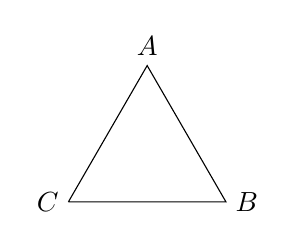
\begin{tikzpicture}
        \node[above](a) at (1,1.73){$A$};
        \node[right](b) at (2,0){$B$};
        \node[left](c) at (0,0){$C$};
        \draw(0,0)--(2,0)--(1,1.73)--(0,0);
    \end{tikzpicture}
    \end{center}
    この三角形の持つ対称性,つまりこの幾何学的対象を「そのままに保つ」ような変換とはなんだろうか.
    もちろん,「何もしない」恒等変換は図形をそのままに保つ.
    他にも,いまあなたが目を閉じている間に,私が三角形を$120\times n$度(ただし$n$は整数)時計回りに回転させても,目を開けたあなたは以前との違いに何も気が付かないだろう.
    その意味で,$120\times n$度回転は正三角形をそのままに保つ変換=対称性である.
    また,それぞれの頂点から対辺の中間地点へとおろした軸に沿って線対称をとっても,図形は変わらない.
    これらの変換,つまり恒等変換$i$,120度,240度の時計回り回転$c_1, c_2$,および点$A, B, C$を通る軸に沿った鏡映反転$\sigma_A, \sigma_B, \sigma_C$は,以下のように頂点を移すが形はそのままに保つ,この正三角形の対称性である.
    \begin{center}
        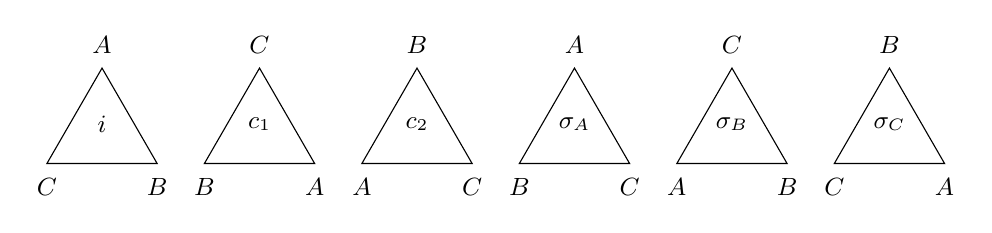
\begin{tikzpicture}[every node/.style={font=\small}]
            \foreach \x in {0,2,4,6,8,10} {
                \draw (\x,0) -- (\x+1.4,0) -- (\x+.7, 1.212) -- cycle;
            }        
            \node at (.7,.5) {$i$};
            \node at (.7,1.5) {$A$};
            \node at (1.4,-.3) {$B$};
            \node at (0,-.3) {$C$};

            \node at (2.7,.5) {$c_1$};
            \node at (2.7,1.5) {$C$};
            \node at (3.4,-.3) {$A$};
            \node at (2,-.3) {$B$};

            \node at (4.7,.5) {$c_2$};
            \node at (4.7,1.5) {$B$};
            \node at (5.4,-.3) {$C$};
            \node at (4,-.3) {$A$};

            \node at (6.7,.5) {$\sigma_A$};
            \node at (6.7,1.5) {$A$};
            \node at (7.4,-.3) {$C$};
            \node at (6,-.3) {$B$};

            \node at (8.7,.5) {$\sigma_B$};
            \node at (8.7,1.5) {$C$};
            \node at (9.4,-.3) {$B$};
            \node at (8,-.3) {$A$};

            \node at (10.7,.5) {$\sigma_C$};
            \node at (10.7,1.5) {$B$};
            \node at (11.4,-.3) {$A$};
            \node at (10,-.3) {$C$};
        \end{tikzpicture}
    \end{center}
    
    これらの対称性$\{i, c_1, c_2, \sigma_A, \sigma_B, \sigma_C\}$は,$i$を単位元とした群をなす.
    まず対称変換を続けて行っても,当然それは対称変換になる,つまりそれは積で閉じており,また積は結合的である.
    $c_1, c_2$が互いを「キャンセル」する逆元であり,また$\sigma_A, \sigma_B, \sigma_C$のそれぞれがそれ自身の逆元になっていることも容易に分かる.
    
    一般に,与えられた図形に対し,その図形をそのままに保つ対称変換の全体は,群を成す.
    そしてこの群は,図形によって変わってくる.
    例えば以下のような二等辺三角形が持つ対称変換は$\{i, \sigma_A\}$の2つである.
    \begin{center}
        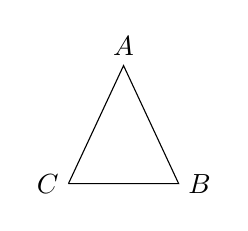
\begin{tikzpicture}
            \node[above](a) at (.7,1.5){$A$};
            \node[right](b) at (1.4,0){$B$};
            \node[left](c) at (0,0){$C$};
            \draw(0,0)--(1.4,0)--(.7,1.5)--(0,0);
        \end{tikzpicture}
    \end{center}
    一方,円の場合はあらゆる角度の回転,および中心点を通るあらゆる軸での鏡映が対称変換になる.
    これは,二等辺三角形よりも三角形が,そして三角形より円のほうがより対称的である,という我々の直観とも合致している.

\end{rei}

\begin{renshu}{}{}
    正三角形の対称性$\{i, c_1, c_2, \sigma_A, \sigma_B, \sigma_C\}$の積表を作れ.(ヒント:もちろん三角形にこれらを適用して結果を逐一確認してもよい.しかしより楽なやり方もある.三角形の変換の一つ一つは,その頂点$\{A, B, C\}$を並び替える置換になっていることに注意せよ.よってその全体は上で見た$S_3$に等しい.)
\end{renshu}
 
\begin{renshu}{}{}
    正方形の対称変換をすべて求め,各変換の逆元を確定せよ.
\end{renshu}

\begin{rei}{クラインの四元群}{klein}
    以上ではカードのシャッフルや図形の変換といった,比較的具体的な例をあげてきたが,最後に抽象的な群の例を一つ見よう.
    以下の積表で定まる群を,クラインの四元群という.
    \[
        \begin{array}{c|cccccc}
                 & i & a & b & c \\ \hline
               i & i & a & b & c \\ 
               a & a & i & c & b \\ 
               b & b & c & i & a \\ 
               c & c & b & a & i \\ 
        \end{array}
    \]
\end{rei}

\begin{rei}{ロボットの操作群}{robot_group}
    前章発展5.1では,ロボットの状態に対するプログラム作用を,その結果の同一性でまとめた同値類$M/\sim$を考えた.
    この同値類は群をなす.
    というのも,以下のような仕方ですべての生成元に対して逆元を考えることができるからだ
    \begin{itemize}
        \item $[a]^{-1} = [bbabb]$ (一歩進む,の逆は右に180度回転・一歩前進・右180度回転),
        \item $[b]^{-1} = [c]$ (右向の逆は左向),
        \item $[c]^{-1} = [b]$ (左向の逆は右向),
        \item $[i]^{-1} = [i]$.
    \end{itemize}
    よってこれらから形成される任意の元,例えば$[baac]$などに対しても,$[baac]^{-1} = [c]^{-1} [a]^{-1} [a]^{-1} [b]^{-1}$といった仕方で逆元が存在する.

    一方で,同値類で割る前の$M$は群ではない.その理由を考えてみよ.
\end{rei}


\section{可換性}
前章では,モノイドにおける重要な区別として可換性を見た.
同様の区分は群においてもそのままで成り立つ.
つまり群$G$が可換であるとは,任意の2つの元$g,h \in G$について$h \circ g = h \circ g$がなりたつことをいう.
これは積表で見ると,表が対角線を中心に対称になっているということだ.
これまでの例で見ると,クラインの四元群は可換だが,$S_3$および正三角形の対称性は可換ではない.


\section{群準同型写像}


\begin{renshu}{}{}
    5章で見た準同型は,群についても同様にいえる.
    群$(G, \circ, i)$から群$(G', \circ', i')$への準同型写像とは,写像$f:G \to G'$であって,すべての$x, y \in G$について$f(x\circ y) = f(x) \circ' f(y)$が成立するものである.
    例えば上の正三角形と二等辺三角形の対象変換の間に,以下のような写像を構築すると,これは両群の間の準同型写像になっている:
    \[
    f(c_1)=f(c_2)=i, \ \ \ f(\sigma_1) = f(\sigma_2) = f(\sigma_3) = \sigma_A.    
    \]
    \begin{enumerate}
        \item これが準同型写像の定義を満たすことを確認せよ.
        \item 上の練習問題で求めた正方形から長方形の対象変換群への準同型写像を構築せよ.
    \end{enumerate}
\end{renshu}


\section{群の作用}

\section{対称性の哲学的含意}

対称性の問題は,陰に陽に,多くの哲学的議論で現れてくる.
またそれだけでなく,対称性は現代の数学・物理学においても非常に重要な概念である.
対称性の重要性が最初に明確に意識されたのは,19世紀後半に数学者のフェリックス・クラインが,弱冠23歳(!)でエルランゲン大学の教授に就任した際に提唱した,エルランゲン・プログラムである.
当時は,19世紀初頭の非ユークリッド幾何学の発見に導かれ,射影幾何学など様々な幾何学が林立していた.
クラインのプログラムは,こうした様々な幾何学を,対称性の観点から分類・統合する,というものである.
そのアイデアをざっくり説明すると,次のようなものである.
\begin{figure}[h]
\begin{center}
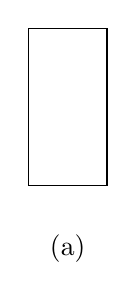
\begin{tikzpicture}
    \draw(0,0)--(1,0)--(1,2)--(0,2)--(0,0);
    \node[below](a) at (0.5,-.5){(a)};
\end{tikzpicture} 
\hspace{2em}
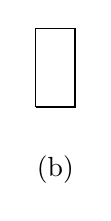
\begin{tikzpicture}
    \draw(0,0)--(0.5,0)--(0.5,1)--(0,1)--(0,0);
    \node[below](b) at (0.25,-.5){(b)};
\end{tikzpicture}
\hspace{2em}
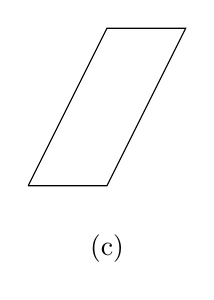
\begin{tikzpicture}
    \draw(0,0)--(1,0)--(2,2)--(1,2)--(0,0);
    \node[below](c) at (1,-.5){(c)};
\end{tikzpicture}
\hspace{2em}
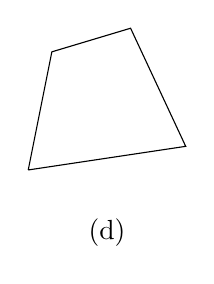
\begin{tikzpicture}
    \draw(0,0)--(2,0.3)--(1.3,1.8)--(0.3,1.5)--(0,0);
    \node[below](d) at (1,-.5){(d)};
\end{tikzpicture}
\hspace{2em}
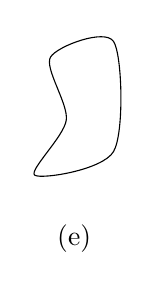
\begin{tikzpicture}
%    \draw plot[smooth cycle] coordinates{(0,0) (1,0) (2,1) (1,2)}
    \draw plot[smooth cycle] coordinates{(0,0) (1,0.3) (1,1.7)(.2,1.5)(.4,.7)};
    \node[below](e) at (.5,-.5){(e)};
\end{tikzpicture}
\end{center}
\caption{幾何学図形(長方形)に対する様々な変換.}
\label{erlangen}
\end{figure}

図\ref{erlangen}の左(a)に書かれた長方形は,様々な幾何学的性質を持っている.
まずそれは線で囲まれており,その線は4本の直線であり,対辺の長さは等しく,隣接した辺同士は直角で交わり,さらには各辺は具体的な長さ(印刷された用紙によって異なるだろうが,例えば長辺3cm)を持っている.
しかしこれらの性質全てが同じステータスを持っているわけではなく,いくつかはより「根源的」であるように思える.
この性質間の質的違いは,対称性の観点から理解できる.
例えば辺の長さは,相似変換によって変わってしまうが,それ以外の性質は不変に保たれる(b).
角度はアフィン変換(affine transformation)と呼ばれる変換により変わるが,対辺の長さが等しいという特徴は保たれる(c).
しかしその特徴も,ある光源から出た光でこの図形を他の面に射影する射影変換(projection transformation)では変わってしまう(d)(プロジェクタから斜めに投影するとスライドの画像がずれてしまうことを思い起こすとわかりやすい).
また最後に,位相のところで見た連続変換を施せば,不変にとどまる性質は「線で囲まれている」ということだけである(e).
これらの変換はそれぞれ,別個の(しかし互いにネストした)群を形成する.
そして上で述べた各性質は,異なる変換群に対する対称性を例示していると考えて良い.
クラインはこうした洞察から,幾何学とは,何らかの変換群に対して不変(invariant)にとどまる性質,すなわち対称性を探求する学問である,と特徴づけた(例えば射影幾何学は,射影変換に対して不変な性質を探求する).

逆に見れば,「幾何学的性質」というものは,変換群に対する対称性として定義することができる.
そして何が正真正銘の幾何学的性質とみなされるかは,扱う幾何学/変換群によって変わってくる.
例えば「角度」という概念は,ユークリッド幾何学では意味があるがアフィン幾何学では意味がない.
したがって,「正三角形」はユークリッド世界では客観的に存在するが,アフィン世界ではそうではない.
このように,性質やモノの実在性を対称性として特徴づけるアプローチは,数学に限らず,物理学でも重要な役割を担ってきた.
例えば古典物理学における物体(古典力学において「存在」するもの)は,ガリレオ変換とよばれる変換群に対して不変性を保つ.
一方,相対論において正真正銘のモノないし性質と認められるものは,それとは別の,ローレンツ変換に対して不変でなければならない.
ローレンツ変換は時間軸と空間軸を「混ぜる」変換なので,例えばものの「長さ」は相対論においては客観的な性質ではない(光速に近い速度で移動すると,同じものが違った長さに見える).

\begin{rei}{有意味性と対称性}{meaningfulness}
京都の平均気温は4月は摂氏14度,8月は28度である.
しかしこれをこれをもって,「京都の8月は4月の2倍暑い」ということは意味をなさない.
というのも気温を華氏で表現すれば,それぞれ57度と82度になり,「2倍」という関係は成立しないからだ.
一般に,温度はアフィン変換$y = \alpha x + \beta$可能\footnote{例えば$y$を華氏,$x$を摂氏とすると,$y = 1.8x+32$.}なので,こうした変換において不変に保たれる性質のみが温度についての客観的性質として認められる.
アフィン変換は群をなすので\footnote{アフィン変換$y=\alpha x + \beta$を$(\alpha, \beta)$で表すと,単位元は$(1,0)$. $(\alpha, \beta), (\alpha',\beta')$という2つの変換に対し,合成は$(\alpha' \alpha, \alpha' \beta + \beta')$. 変換$(\alpha, \beta)$の逆元は$(1/\alpha, -\beta)$. 結合律については明らか.},これは対称性である.
ここから,ある対象(温度)についてどんな言明が有意味であるかは,その対象の対称性,すなわちそれが許容する変換群を定めればよい,という方針が従う.
これは測定理論(theory of measurement)の中心的な考え方である\citep[e.g,][]{Narens2007-ty}.
\end{rei}


\begin{rei}{対称性議論:逆転クオリア}{inverse_qualia}
逆に,対称変換は対象の本質を変えないのであるから,そうした変換によって変わるような性質は,実在的ないしは客観的な性質ではない,という議論戦略も存在する.そうした議論は一般に\emph{対称性議論}(symmetry argument)と総称される.
有名な対称性議論として\emph{逆転クオリア}(inverted qualia)がある.
通常の人間が「赤」と感じる波長の光を見ると,「緑」に見えるような人を考えよう.
そうした人は,我々が木の葉を見るときに感じる質感を熟れたリンゴを見るときに感じており,また逆もしかりであるが,しかし行動においては全く差異を見いだせないだろう(むしろクオリアが逆転しているのは\emph{あなた}かもしれない).
これは,「今,赤(緑)の質を感じている」という性質を互いに入れ替えるような変換(これは群である)は,人間の状態一般を不変に保つ対称性変換であるということである.
よってそうした変換において変化する性質は,実在的な性質ではない,したがってクオリアについての事実は存在しない.
これはクオリアについての対称性議論である.
\end{rei}

\begin{rei}{対称性議論:グルーパラドクス}{grue}
今まで観測されたエメラルドはすべて緑greenであったとしよう.
ここから,「全てのエメラルドは緑である」と考えるのは妥当な帰納推論であるように思える.
しかしいま,「2025年以前に観測され緑であるものと,2025年以降に観測され青であるもの」を指すグルーgrueという述語を導入する.
すると今までに観測されたエメラルドはすべてグルーなので,「全てのエメラルドはグルーである」という仮説も同様に支持されそうに思えるが,これは明らかにおかしい.
一つの解決策は,「2025年」という特定の時間を含む述語はおかしい,と考えることかもしれない.
しかしいま,「2025年以前に観測され青であるものと,2025年以降に観測され緑であるもの」を指すブリーンbleenという述語を導入しよう.
すると述語「緑」は,「2025年以前に観測されグルーであるものと,2025年以降に観測されブリーンであるもの」というように定義し返される.つまりグルー/ブリーンを使う人からすれば,「緑」のほうこそ特定の時間を含んでしまっている!
これは\cite{Goodman1955-nr}によって提唱された,\emph{グルーパラドクス}と呼ばれる帰納推論の未解決問題である.
これは緑/青という述語と,グルー/ブリーンという述語は互いに変換可能であり,よって緑仮説とグリーン仮説では優劣をつけることができないはずだという,対称性議論として理解できる.
\end{rei}

\begin{rei}{還元主義}{reductionism}
我々は上で,考える対称性の違いにより幾何学的性質の「根源性」の度合いのようなものが考えられることを見た.
そして現代物理学において,実在的性質は対称性,つまり変換群に対する不変性として定義されることを見た.
同じようなことは,他の科学にもいえるだろうか.
例えば,何らかの変換群に対する不変性として化学的性質,生物学的性質,などを定義していくことは可能だろうか.

またさらに,そのように定義されたとき,それぞれの変換群は幾何学のときのような階層構造を持っているだろうか.
例えば,化学的・生物学的性質はローレンツ変換に対しては不変だと期待できるかもしれない(なぜならそれは物理的性質を不変に保つのだから).
同じように,生物学的性質は化学的変換に対して不変だろうか.
存在論的還元主義は,この問いに肯定的に答える:すなわちそれによれば,各科学分野における客観的性質は,その分野を特徴付ける変換群によって定義され,なおかつその変換群は階層的な構造を持っている.
\end{rei}

\begin{renshu}{}{}
上で述べた変換群の階層構造を,群準同型の言葉で表わせ.
また群準同型が半順序を成すという練習問題5.3の結論は,還元主義的科学観に対しどのような含意を持つだろうか.
\end{renshu}

\begin{renshu}{}{}
還元主義に従い,ミクロ理論$T$の性質を特徴づける変換群$f$からマクロ理論$T'$の変換群$g$への準同型写像があると仮定しよう.
このとき,$T$と$T'$の性質の間にはどのような関係が成り立っているだろうか.
具体的には,準同型写像の存在は$T'$の性質が$T$の性質に付随(supervene)することを含意するだろうか.
また逆に,付随性が満たされるとき,$f$から$g$への準同型写像が存在するだろうか.
\end{renshu}


\bibliographystyle{apalike}
\bibliography{m4p}

\end{document}